\documentclass[11pt,letterpaper]{article}

\usepackage[margin=1in]{geometry}
\usepackage{amsmath,amssymb,amsthm,mathtools}
\usepackage{booktabs}
\usepackage{array}
\usepackage{enumitem}
\usepackage[protrusion=true,expansion=false]{microtype}
\usepackage{xcolor}
\usepackage{tcolorbox}
\tcbuselibrary{skins,breakable}
\usepackage{caption}
\usepackage{titlesec}
\usepackage{fancyhdr}
\usepackage{listings}
\usepackage{graphicx}
\usepackage{tabularx}
\usepackage{tikz}
\usetikzlibrary{positioning,arrows.meta,decorations.pathreplacing,calc,shapes.geometric,backgrounds,fit}
\usepackage[colorlinks=true,linkcolor=violet,urlcolor=violet,citecolor=violet]{hyperref}
\hypersetup{
  pdftitle={The Witting Reference Fabric: An Ultimate Computer Architecture},
  pdfauthor={Wil Dahn},
  pdfsubject={A hardware/software architecture for referenceable ASI-scale compute},
  pdfkeywords={ASI, computer architecture, Witting Reference Fabric, UOR, HLIX, Oko, Smart Assets}
}

% ============ Theorem environments ============
\newtheorem{theorem}{Theorem}
\newtheorem{proposition}[theorem]{Proposition}
\newtheorem{corollary}[theorem]{Corollary}
\newtheorem{definition}[theorem]{Definition}
\newtheorem{lemma}[theorem]{Lemma}
\theoremstyle{remark}
\newtheorem{remark}[theorem]{Remark}
\newtheorem{claim}[theorem]{Claim}

% ============ Substrate shorthand ============
\newcommand{\W}{W(3,3)}
\newcommand{\Sp}{\mathrm{Sp}}
\newcommand{\Aut}{\mathrm{Aut}}
\newcommand{\Stab}{\mathrm{Stab}}
\newcommand{\FF}{\mathbb{F}}
\newcommand{\ZZ}{\mathbb{Z}}
\newcommand{\CC}{\mathbb{C}}
\newcommand{\Atlas}{\mathrm{Atlas}_{12288}}
\newcommand{\Rsix}{R_{96}}
\newcommand{\TPS}{\mathrm{TPS}}
\newcommand{\BoseMesner}{\mathcal{B}}
\newcommand{\UOR}{\mathrm{UOR}}
\newcommand{\HCP}{\mathrm{HCP}}
\newcommand{\ket}[1]{\lvert #1\rangle}

% ============ Section formatting ============
\titleformat{\section}{\Large\bfseries\color{violet!60!black}}{\thesection}{0.7em}{}
\titleformat{\subsection}{\large\bfseries\color{violet!50!black}}{\thesubsection}{0.7em}{}
\titleformat{\subsubsection}{\bfseries\color{violet!45!black}}{\thesubsubsection}{0.7em}{}

% ============ Headers ============
\pagestyle{fancy}
\fancyhf{}
\fancyhead[L]{\small\itshape Witting Reference Fabric}
\fancyhead[R]{\small\thepage}

% ============ Listings ============
\definecolor{codebg}{HTML}{F7F4FA}
\lstdefinestyle{plain}{
  basicstyle=\ttfamily\small,
  backgroundcolor=\color{codebg},
  frame=single,
  framerule=0.3pt,
  rulecolor=\color{violet!50!black},
  columns=fullflexible,
  keepspaces=true,
  showstringspaces=false,
  breaklines=true,
  keywordstyle=\color{violet!70!black}\bfseries,
}
\lstset{style=plain}

% ============ Boxes ============
\newtcolorbox{keyresult}[1][]{
  colback=violet!5!white,
  colframe=violet!60!black,
  fonttitle=\bfseries,
  title={#1},
  arc=2pt,
  boxrule=0.5pt,
  breakable
}
\newtcolorbox{thesis}{
  colback=yellow!5!white,
  colframe=orange!70!black,
  arc=2pt,
  boxrule=0.5pt,
  left=8pt,right=8pt,top=6pt,bottom=6pt,
  breakable
}
\newtcolorbox{plainenglish}[1][]{
  colback=cyan!5!white,
  colframe=cyan!60!black,
  fonttitle=\bfseries\color{black},
  title={#1},
  arc=2pt,
  boxrule=0.4pt,
  breakable,
  left=8pt, right=8pt, top=4pt, bottom=4pt
}
\newtcolorbox{intuition}[1][]{
  colback=green!4!white,
  colframe=green!50!black,
  fonttitle=\bfseries\color{black},
  title={#1},
  arc=2pt,
  boxrule=0.4pt,
  breakable,
  left=8pt, right=8pt, top=4pt, bottom=4pt
}
\newtcolorbox{designprinciple}[1][]{
  colback=violet!4!white,
  colframe=violet!50!black,
  fonttitle=\bfseries,
  title={#1},
  arc=2pt,
  boxrule=0.4pt,
  breakable
}
\newtcolorbox{connection}{
  colback=gray!7!white,
  colframe=gray!50!black,
  arc=2pt,
  boxrule=0.3pt,
  left=8pt, right=8pt, top=4pt, bottom=4pt
}
\newtcolorbox{bluf}[1][]{
  colback=blue!4!white,
  colframe=blue!55!black,
  fonttitle=\bfseries,
  title={#1},
  arc=2pt,
  boxrule=0.5pt,
  left=8pt, right=8pt, top=5pt, bottom=5pt,
  breakable
}
\newtcolorbox{guardrail}[1][]{
  colback=red!3!white,
  colframe=red!45!black,
  fonttitle=\bfseries,
  title={#1},
  arc=2pt,
  boxrule=0.4pt,
  left=8pt, right=8pt, top=5pt, bottom=5pt,
  breakable
}

\title{\vspace{-1.3cm}\textbf{The Witting Reference Fabric}\\[3pt]
\Large An Ultimate Hardware/Software Computer Architecture:\\
Content-Addressed Memory, Projection-Native Execution,\\
Network-Fabric Consensus, and Smart-Asset Economics at $70$M~TPS over $10^9$ Nodes}

\author{Wil Dahn\\
\normalsize\textit{Witting Reference Fabric Project}\\
\normalsize\textit{In collaboration with the UOR Foundation, Oko, Smart Assets, DTR/HLIX}}

\date{June 2026 \hspace{1em}\textit{v2 architecture edition}}

\begin{document}
\maketitle

\vspace{-0.6cm}
\begin{abstract}
\noindent
Artificial superintelligence (ASI) is usually framed as a model-scale problem: more
parameters, more accelerators, more data centres. This paper frames it as a substrate
problem. If HLIX turns infrastructure into a projection--execution--emission cycle, UOR
turns objects into universal content-derived references, Oko supplies network-fabric
Byzantine finality, and Smart Assets attach economics to workloads, then the missing
piece is an architecture that makes one billion heterogeneous nodes behave like one
referenceable compute object.

Assume the supervisor's target: $70$\,M aggregate transactions per second over a
$10^9$-node mesh and a $70$B-parameter ASI workload as the benchmark class. The proposed
\textbf{Witting Reference Fabric} interprets that mesh as a layered hardware/software
fabric: UOR supplies typed content addresses; HLIX supplies projection-native scheduling;
Oko supplies hard-final network consensus; Smart Assets supply programmable economics;
and the W(3,3) / Witting finite geometry supplies a compact coordination lattice with
$40$ address classes, $240$ carrier links, $480$ directed routes, $51{,}840$ finite
control symmetries, and an $11$-branch non-backtracking transport rule. The architecture
also admits a stronger memory primitive: a \emph{referenceable flow cell}, where the
stored object is not a resting byte pattern but the canonical invariant of a bounded
repeatable trace.

The architecture's natural information density is $\boxed{3/8 = q/2^q}$, appearing
exactly as the $R_{96}/256$ Atlas compression ratio and the W(3,3) chiral eigenspace
fraction $15/40$. The native CSS storage layer sits just below it at
$81/240 = 27/80$, spending the $3/80$ gap as protection overhead. The natural cadence is
$j(i)=1728=k^3$ orbit-cycles per
consensus epoch, so $70$\,M~TPS induces $1.21\times 10^{11}$ substrate cycles/sec. A
$40^6 = 4.096$ billion-node fractal deployment exceeds the $10^9$-node target with
redundancy. The central implication is architectural: ASI-scale compute becomes
referenceable, auditable, sovereign, self-coordinating, and economically addressable at
planetary scale.
\end{abstract}

\begin{bluf}[Bottom line]
\noindent\textbf{The Dahn thesis:}
\emph{ASI becomes governable only when compute, memory, identity, provenance, consensus,
and economics share the same reference substrate.} In this paper the substrate is
Atlas-$12288$ / UOR; the operating cycle is HLIX/HCP projection--execution--emission; the
coordination fabric is Oko's BIER/BLA network consensus; the workload unit is the Smart
Asset; and the compact control geometry is $\Aut(\W)=\Sp(4,\FF_3)=W(E_6)$.
\end{bluf}

\begin{guardrail}[Scope]
This is an architecture and strategy paper, not a claim that ternary Witting silicon or
Bell-qutrit storage already exists as production hardware. The near-term path is to use
the Witting finite geometry as coordination and verification mathematics for
HLIX/UOR/Oko software systems, then progressively harden the same invariants into
accelerators, storage, and fabric. The flow-cell experiments cited below are finite
software harnesses over W(3,3), not measured device noise results.
\end{guardrail}

\tableofcontents
\vspace{6pt}\hrule\vspace{8pt}

% ===========================================================================
\section{Introduction: From Opaque ASI to Referenceable Compute}
% ===========================================================================

\begin{plainenglish}[Plain-English summary]
The question is not merely whether ASI can be made smarter. The question is whether an
ASI-grade system can be made \emph{referenceable}: can we name every piece of compute,
verify every output, preserve every receipt, route work across one billion nodes, and keep
sovereign control over data without centralizing the whole system? The answer proposed
here is yes, if the HLIX/UOR/Oko/Smart-Assets stack is underpinned by a finite control
geometry that can route, audit, and compress without becoming the subject of the paper.
\end{plainenglish}

\subsection{Why ASI makes architecture a governance problem}

Computer architecture has not changed structurally since John von Neumann sketched the
stored-program model in 1945. Pipelining, caches, out-of-order execution, SIMD, and GPGPU
acceleration are all improvements on the same scaffold: a central processor fetches
instructions and data from separate memory over a shared path and executes them according
to local state. For ordinary software this is an efficiency problem. For ASI it becomes a
governance problem: the same bottleneck that hides memory locality also hides provenance,
coordination, jurisdiction, and accountability.

In 2026 we sit at a triple convergence of stress on this scaffold:
\begin{enumerate}[leftmargin=2em,nosep]
\item \textbf{Monolithic die scaling has ended.} Chiplet packaging admits architectural
defeat: we can no longer make a single chip bigger.
\item \textbf{Memory bandwidth lags compute by} $\mathbf{100\times}$. CPU FLOPs grow at
roughly $1.4\times$ per year; DRAM bandwidth grows at roughly $1.07\times$ per year. We
are paying for compute we cannot feed.
\item \textbf{Distributed computing is now the workload, not a special case.}
Cross-datacentre, cross-jurisdiction, cross-vendor coordination is the norm, but the
underlying architectures still pretend the bus model holds.
\item \textbf{AI turns logs into liability.} An ASI workflow is not a single inference call;
it is a chain of retrieval, planning, tool use, delegation, payment, and post-hoc audit.
If those events are not first-class addressable objects, the system cannot be trusted.
\end{enumerate}
The retrofits accumulate: virtual memory hides the physical memory; cache hierarchies hide
the memory bus; transactional memory hides shared-memory races; distributed-systems
protocols hide the network behind RPC. Every retrofit costs latency, complexity, energy,
and trust. The industry calls this ``the memory wall'' or ``the dark-silicon problem.''
What it actually is, structurally, is the cost of fifty years of layering retrofits on
top of a 1945 architecture.

\subsection{Four convergent stacks}

Four independent recent stacks each chip away at one piece of the ASI substrate problem:

\begin{itemize}[leftmargin=2em]
\item \textbf{Oko} (the network-fabric Byzantine Lattice Agreement consensus protocol)
eliminates the leader-based quadratic bottleneck of classical BFT. Instead of $n$ nodes
exchanging $O(n^2)$ messages, Oko uses BIER multicast at the network layer: virtual
switches replicate packets to a $55$-validator committee with $O(n)$ aggregate
communication. The simulator measures $12$\,M~TPS per server at fixed committee size, with
linear scaling in per-server compute; the supplied source pack projects billion-plus
aggregate TPS by clustering servers behind the same committee invariant
\cite{oko-threepager,okopipi-l1}. Throughput is now a per-server parameter, not a
validator-count parameter.
\item \textbf{The UOR Foundation} (Universal Object Reference) defines a content-addressed
substrate: one content-derived address per object, persistent identity, trustless
verification, and universal composability. The current public site presents UOR as a
unified computational substrate for agentic AI with $14$ namespaces, $82$ classes, and
$120$ properties \cite{uor-site}; the current UOR-Framework repository reports version
$0.5.2$ with $34$ namespaces, $474$ classes, $948$ properties, and $3601$ named
individuals \cite{uor-framework}. The crown jewel for this paper is the Atlas-$12288$
frame: $48$ pages of $256$ bytes, with an $R_{96}$ resonance classification compressing
the byte alphabet onto $96$ classes.
\item \textbf{HLIX} (Hybrid Linked Infrastructure Xchange) operationalises the HCP
\emph{projection cycle}---every system event is a \emph{projection} (a declarative
description of what should happen) that triggers an \emph{execution} on a substrate node,
emitting a new content-addressed result plus a verifiable receipt. HLIX targets $1$\,billion
nodes across the ``HexaScaler'' axes of Cloud, Edge, Mesh, AI, Chain, and Sovereign
\cite{hlix-hcp}.
\item \textbf{Smart Assets} turn workloads into economic objects: CPU/GPU/NPU time,
models, datasets, receipts, services, and governance shares become fundable, billable,
tradeable compute assets. In the source image, the attributes are explicitly modular,
decentralised, composable, interoperable, programmable, transferable, and incentive
aligned. In ASI terms, Smart Assets are how autonomous work pays for itself without
ceding coordination to a central owner.
\end{itemize}

\subsection{Implementation grounding from the UOR code}

This paper treats UOR as an implementation surface, not only as a concept. The repository
review matters because the architecture should be buildable in stages:

\begin{center}
\renewcommand{\arraystretch}{1.15}
\begin{tabularx}{\linewidth}{>{\raggedright\arraybackslash\bfseries}p{0.21\linewidth}>{\raggedright\arraybackslash}X}
\toprule
\textbf{Repository} & \textbf{Architectural role imported here} \\
\midrule
UOR-Framework &
Rust ontology workspace for content-addressed, symmetric, multi-metric object spaces
based on $Z/(2^n)Z$, with generated Rust and Lean surfaces plus conformance gates
\cite{uor-framework}.\\
uor-addr &
Typed reference vocabulary producing deterministic \texttt{sha256:<64hex>} labels from
canonical bytes: JSON via RFC~8785 JCS, S-expressions, XML-C14N, DER ASN.1, code-module
ASTs, ring elements, GGUF, ONNX, and schema-pinned descendants. The core is
\texttt{no\_std}; several realizations are \texttt{no\_alloc} \cite{uor-addr}.\\
prism &
Standard-library facade for UOR axes, including cryptographic hash axes
SHA-2/3, BLAKE3, Keccak, signature axes, and commitment axes \cite{uor-prism}.\\
atlas-12288 &
C/Lean hybrid FFI exposing the constants this paper uses directly:
\texttt{UOR\_PAGES()=48}, \texttt{UOR\_BYTES()=256}, and
\texttt{UOR\_RCLASSES()=96}, with Lean-backed and pure-C modes \cite{uor-atlas}.\\
\bottomrule
\end{tabularx}
\end{center}

\subsection{Our finding}

\begin{intuition}[The convergence]
\emph{Fast consensus, universal addressing, sovereign orchestration, and workload
economics all point toward the same missing layer.} Oko says coordination must live in the
network fabric. UOR says identity must be content-derived. HLIX says infrastructure must
be projected and receipted. Smart Assets say compute must be economically addressable. The
Witting Reference Fabric supplies the finite hardware/software control architecture that
lets these four claims compose.
\end{intuition}

The architectural fixed point is the \textbf{Witting polytope}---the unique $40$-vertex
configuration on which the symplectic polar space $\W$ is canonically realised---with
automorphism group $\Sp(4,\FF_3) \cong W(E_6)$ of order $51{,}840$. The Witting polytope
was discovered by Hermann Witting in $1937$ as a uniform polychoron in $\CC^4$. This paper
treats it as the organising candidate for a substrate-coherent ASI fabric: small enough to
compile, symmetric enough to coordinate, and rigid enough to audit.

\subsection{What this paper claims}

We do \emph{not} claim that the Witting Reference Fabric is a marginal improvement over Von
Neumann. We claim that it is a different basin of attraction in the architecture design
space, in which the following retrofits are replaced by substrate-native primitives:

\begin{itemize}[leftmargin=2em,nosep]
\item No bus---communication is intrinsic to the topology, not a separate channel.
\item No cache hierarchy---the substrate's spectrum supplies the cache levels exactly.
\item No ISA accretion---the instruction set is finite by construction (exactly $30$
families).
\item No bolted-on ECC goal---the base CSS carrier and protected lift are designed into
the storage path.
\item No separate networking---on-chip and off-chip use the same fabric protocol.
\item No unanchored cryptography---addressing is cryptographically pinned, while
signatures and post-quantum policy remain explicit.
\item No separate consensus---BLA is the thread-coordination primitive.
\item No root user---identity is structural (the stabiliser subgroup).
\item No hidden ASI state---agent memory and tool use become receipt-bearing objects.
\end{itemize}

The paper unfolds in six movements. \S\ref{sec:asi} gives the executive answer for ASI.
\S\ref{sec:axioms} states the seven design axioms. \S\ref{sec:atlas} explains the
Atlas-$12288$ memory frame and the universal-density reading. \S\ref{sec:hw} describes the
hardware path (Witting tile, three-channel bus, spectral cache, Bell-qutrit storage, BIER
fabric). \S\ref{sec:isa} explains the group-action ISA. \S\ref{sec:os} describes the
projection operating system. The remaining sections quantify performance, address
security and trust, and lay out the deployment roadmap.

% ===========================================================================
\section{Executive Answer: Why This Architecture Matters for ASI}\label{sec:asi}
% ===========================================================================

\begin{bluf}[The highest-level implication]
The Witting Reference Fabric does not merely make ASI faster. It makes ASI
\emph{legible at substrate scale}. The W(3,3) / Witting layer supplies a finite coordinate
system in which every agent action can be named, routed, receipted, compared, composed,
and paid for without collapsing the network into a central scheduler.
\end{bluf}

\begin{center}
\renewcommand{\arraystretch}{1.18}
\begin{tabularx}{\linewidth}{>{\raggedright\arraybackslash\bfseries}p{0.25\linewidth}>{\raggedright\arraybackslash}X}
\toprule
\textbf{ASI requirement} & \textbf{Architecture contribution} \\
\midrule
Referenceable cognition &
Every model, prompt, memory, tool call, policy, dataset, and receipt becomes a UOR object
with a stable content-derived address. The ASI's cognition is not hidden in a vendor log;
it is a traversable object graph.\\
Verifiable inference &
HLIX emissions attach receipts to outputs; Oko finalises them; the Witting control plane
gives the receipts an invariant coordinate system. The question changes from ``do we trust
this answer?'' to ``which orbit produced this answer, from which inputs, under which
policy?''\\
Billion-node coordination &
Oko keeps consensus committee size fixed while per-server work scales; HLIX schedules
projections across heterogeneous nodes; W(3,3) supplies a finite symmetry vocabulary for
coordinating work without a single global scheduler.\\
Sovereignty by construction &
Raw data can remain local while proofs move globally. Jurisdictional control is handled by
policy containers and receipt chains, not by manually negotiated integrations.\\
Persistent ASI memory &
The HCP Container Store becomes long-horizon memory: immutable resources, references,
views, datasets, and receipts. The architecture adds the compression and orbit structure
needed to keep that memory coherent rather than merely large.\\
Economic agency &
Smart Assets attach funding, billing, ownership, and rewards to workloads. ASI agents can
commission compute, prove delivery, and settle usage without a trusted platform operator.\\
Failure containment &
Stabiliser-based identity and orbit histories make anomalies detectable: forged outputs,
policy drift, prompt-injection residues, and contradictory provenance become graph defects
rather than subjective review findings.\\
\bottomrule
\end{tabularx}
\end{center}

\begin{figure}[ht]
\centering
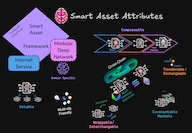
\includegraphics[width=0.72\linewidth]{assets/SA_Attributes.png}
\caption{Smart Asset attributes from the provided source image \cite{smart-assets-image}.
In this architecture a
Smart Asset is the economic envelope around a referenceable workload: modular, composable,
incentive-aligned, transferable, and executable across the HLIX/Oko/UOR mesh.}
\label{fig:smart-assets}
\end{figure}

\begin{connection}
\textbf{The ASI translation.} UOR answers ``what is this object?'' HLIX answers ``where
can this projection execute?'' Oko answers ``when is this state final?'' Smart Assets
answer ``who pays and who is rewarded?'' The Witting Reference Fabric answers ``which
invariant hardware/software structure makes all of those answers compose without losing
meaning?''
\end{connection}

\subsection{The imported W33 control ledger}

The paper imports the local W33/Witting work as a control ledger, not as a physics thesis.
The useful facts are finite, testable architecture constants:

\begin{center}
\renewcommand{\arraystretch}{1.15}
\begin{tabularx}{\linewidth}{>{\raggedright\arraybackslash\bfseries}p{0.22\linewidth}>{\raggedright\arraybackslash}X}
\toprule
\textbf{Constant} & \textbf{Architecture meaning} \\
\midrule
$40$ &
Reference classes / tile cores / Sylow-$3$ handles.\\
$240$ &
Undirected carrier links; base edge-code carrier.\\
$480$ &
Directed forward/return carrier slots.\\
$51{,}840$ &
Finite control symmetries $\Aut(\W)$; small enough for lookup-table scheduling.\\
$30$ &
Conjugacy classes; instruction-family count and control vocabulary.\\
$1+24+15$ &
Bose--Mesner channel split: broadcast, working set, persistent/chiral state.\\
$39+120+81=240$ &
QEC/photonic ledger partition preserving the $81$-state logical tail.\\
$240\cdot 7^3=82{,}320$ &
Protected Steane/$\Phi_6$ lift used as the active protection target beyond the base
$d_Z=4$ carrier.\\
$p_{\mathrm{Ih}}=11$ &
Non-backtracking fabric branch used for routing and multicast intuition.\\
\bottomrule
\end{tabularx}
\end{center}

The ledger is deliberately operational: it tells a compiler, scheduler, storage
controller, or network switch what finite object it is using. It does not ask the reader
to accept a Theory-of-Everything claim before evaluating the architecture.

% ===========================================================================
\section{The Seven Design Axioms} \label{sec:axioms}
% ===========================================================================

\begin{plainenglish}[Plain-English summary]
A good architecture has a small number of \emph{design principles}---rules every part of
the system obeys. Below are seven. Each replaces a convention from 1945 with something
the math says is better. Read them quickly first; subsequent sections will derive each
one in detail.
\end{plainenglish}

\begin{designprinciple}[A1: Content-Address Everything]
Every datum---memory cell, register, instruction, message, process, file---has a single
canonical address derived from its content by the $\psi$-pipeline: a deterministic
canonicalisation followed by Blake3 (or sha256) hashing. No location-based addresses
exist anywhere in the system.
\end{designprinciple}

\begin{designprinciple}[A2: Compute Is Group Action]
The only operation available to a process is the action of an element of $\Aut(\W) =
W(E_6)$ on an edge-mode configuration $\mathcal{C} \subseteq E(\W)$. There is no separate
ALU, control unit, branch unit, or vector unit. Arithmetic, control flow, and parallelism
are specialisations of the same group action.
\end{designprinciple}

\begin{designprinciple}[A3: Spectral Cache Replaces Heuristic Cache]
Cache hierarchy is the spectral decomposition of the W(3,3) adjacency operator
$A = k E_0 + r E_1 + s E_2$, with three projectors $E_0, E_1, E_2$ of ranks
$\{1, 24, 15\}$ acting as three native cache levels. Cache replacement is
substrate-forced, not heuristic.
\end{designprinciple}

\begin{designprinciple}[A4: Storage Is Trace-Locked]
Static objects are content-addressed by UOR CIDs. Active memory cells are
trace-addressed: the physical state keeps moving, while the stored datum is
$\mathrm{CID}_{\rm flow}=H(\mathrm{canon}(x_0,x_1,\ldots,x_T))$, the canonical invariant
of a bounded repeatable trace. A temporal Bell qutrit is the far-horizon physical storage
cell; a W33 non-backtracking flow cell is the software-first primitive.
\end{designprinciple}

\begin{designprinciple}[A5: BIER Multicast Is the Fabric]
There is no bus. Every core has $k=12$ direct neighbours plus $q^q = 27$ disjoint
reachable cores. All communication is BIER multicast through embedded virtual switches;
fabric bandwidth scales linearly with core count.
\end{designprinciple}

\begin{designprinciple}[A6: CSS Code Is Native ECC]
The CSS code $[[\,|E|, q^{q+1}, \mu, q\,]]_3 = [[240, 81, 4, 3]]_3$ is hardwired into the
memory frame. Logical-to-physical ratio $27/80 = q/2^q = 3/8$.
\end{designprinciple}

\begin{designprinciple}[A7: Identity Is a Stabilizer Subgraph]
A process, user, or container has no UID, no PID, no root capability. Its identity is
the subgroup $\Stab_{\Aut(\W)}(\mathcal{C})$ of automorphisms fixing its edge-mode
configuration. Provenance is the orbit history; trust is the orbit signature.
\end{designprinciple}

\begin{connection}
\textbf{How the axioms connect.} A1 (content addressing) makes A2 (group-action compute)
work because the group acts on \emph{content}, not locations. A2 makes A3 (spectral
cache) work because the spectral decomposition is a property of the group action. A3
makes A4 (Bell-qutrit storage) practical because the spectrum exactly matches the
single-qutrit state space. A4 makes A6 (CSS code) practical because persistent state has
a canonical trace witness that can be syndromically repaired. A5 (BIER multicast) makes A2 work at scale because group action
must be broadcast. A7 (stabiliser identity) makes A1 trustworthy because identity is
substrate-coherent. Every axiom supports every other; none is layered on.
\end{connection}

% ===========================================================================
\section{The Atlas-12288 Memory Frame: The Universal Unit}\label{sec:atlas}
% ===========================================================================

\begin{plainenglish}[Plain-English summary]
Memory in our architecture is not byte-addressed. It is organised into \emph{frames} of
exactly $12288$ bytes. Each frame is a $48$-page $\times$ $256$-byte table. Each
$256$-byte page is then compressed by a fixed mapping into one of $96$ equivalence
classes (the $R_{96}$ classification). These numbers---$12288$, $48$, $256$, $96$---are
not arbitrary; the UOR Foundation chose them on entirely different grounds, and they
\emph{all} land on the same five-prime substrate alphabet, and the compression ratio
$96/256 = 3/8$ is \emph{also} the rate of our error-correcting code and \emph{also} a
natural eigenvalue fraction of the underlying graph. We call this the Universal Density
Theorem.
\end{plainenglish}

\subsection{What UOR actually built}

UOR's atlas-12288 reference implementation (C with Lean 4 verification) treats every
addressable resource as a frame of $12288$ bytes structured as:
\begin{itemize}[leftmargin=2em,nosep]
\item $48$ \emph{pages}, each $256$ bytes long (so $48 \times 256 = 12288$),
\item an \emph{$R_{96}$ classifier} mapping each page's $256$ possible byte values to one
of $96$ resonance classes,
\item \emph{conservation-budget checks} (\.{$\alpha_4 \alpha_5 = 1$}, from which the $48$
arises as a unity constraint),
\item canonical encode/decode (sha256-addressable).
\end{itemize}
The team described the result as ``$3/8$ compression'' ($96 / 256 = 0.375$). They were
matter-of-fact about it. They did not (in the public materials) state why $48$, $256$, or
$96$; they were simply the numbers that fell out of the unity constraint and the desired
information density.

\subsection{The substrate reading}

Set $q = 3$ (ternary), $\mu = 4$ (spacetime), $F_5 = 5$ (smallest post-$q$ prime),
$\Phi_3 = 13$, $\Phi_6 = 7$ (cyclotomic values at $q$). Then:
\begin{align*}
48     &\;=\; q! \cdot 2^q                       &\text{(pages per frame)}\\
256    &\;=\; \mu^4 \;=\; 2^{\Phi_6 + 1}          &\text{(bytes per page; the dS identity)}\\
96     &\;=\; 2^{F_5} \cdot q                     &\text{($R_{96}$ resonance classes)}\\
12288  &\;=\; q! \cdot 2^{q + \Phi_6 + 1}         &\text{(frame size)}\\[2pt]
\frac{96}{256} &\;=\; \frac{q}{2^q} \;=\; \frac{3}{8} &\text{(natural density)}
\end{align*}
All four Atlas constants land on substrate primitives, with no constant in the architecture
drawing on any prime outside the five-element substrate alphabet. The compression ratio
$3/8$ is independently the fraction $g/v = 15/40$ of the chiral eigenspace of the W(3,3)
adjacency operator. The base CSS carrier $[[240, 81, d_Z=4]]_3$ sits nearby at
$81/240 = 27/80$, using the $3/80$ gap between $27/80$ and $3/8$ as storage-protection
overhead. \emph{The fabric density is exact; the protected-storage layer deliberately
spends a small part of it.}

\begin{keyresult}[The Universal Density Theorem]
The natural information density of a $\Sp(4,\FF_3)$-equivariant content-addressed
computer is $\boxed{q/2^q = 3/8}$. This density is realised exactly by:
\begin{enumerate}[label=(\roman*),leftmargin=2em,nosep]
\item the UOR Atlas resonance compression ratio $R_{96}/2^8$,
\item the chiral-eigenspace fraction $g/v$ of the W(3,3) adjacency spectrum.
\end{enumerate}
The native CSS storage layer then runs at $27/80$, exactly $3/80$ below the fabric density,
which is the architecture's protection budget rather than a failed match.
\end{keyresult}

\begin{intuition}[Why $3/8$ feels right]
Think of $q/2^q$ as ``three things in a space of eight.'' A ternary alphabet (three
symbols) embeds into a binary alphabet (eight $3$-bit slots) with three slots holding
real information and five slots holding the redundancy that lets you correct errors.
That ratio appears wherever the substrate makes a choice between density and resilience.
\end{intuition}

\subsection{What an address looks like}

A compact $64$-bit WRF reference-class handle is sized by
\[
\underbrace{2^{64}}_{\text{handle space}}
\;=\;
\underbrace{40}_{\text{Sylow-3 vertex}}
\,\cdot\,
\underbrace{1{,}296}_{|N_G(P_3)| \text{ normaliser}}
\,\cdot\,
\underbrace{2^{48.34}}_{\text{contingent payload, approx.}}.
\]
The first factor (the $40$ Witting vertices) corresponds to the $40$ Sylow-$3$ subgroups
of $\Aut(\W)$ by Theorem~\ref{thm:syl}; the second (the $1{,}296$-element normaliser) is
fixed at the vertex; the residual $\approx 48.34$ bits encode the frame's contingent
payload. This is a compact execution handle; canonical UOR identity remains the
content-derived CID.

\begin{theorem}[Hidden Sylow Address Bijection]\label{thm:syl}
$n_3(\Sp(4,\FF_3)) = v = 40$. The $40$ Witting vertices are in canonical bijection with the
$40$ Sylow-$3$ subgroups of $\Aut(\W)$. Every WRF object handle selects a unique
Sylow-$3$ coset of $\Aut(\W)$.
\end{theorem}

The structural consequence is that ``where'' an object lives in the address space is
algebraically constrained by ``what'' it is: there is no separate ``placement policy.''
The substrate places it.

% ===========================================================================
\section{Hardware: The Witting Substrate}\label{sec:hw}
% ===========================================================================

\begin{plainenglish}[Plain-English summary]
The physical chip is built from \emph{tiles}. Each tile holds $40$ small computing cores
arranged in a precise mathematical shape called the Witting polytope. Inside each tile
the cores talk to each other via three specialised buses (not one). Between tiles, chips,
or even continents, the same fabric protocol carries traffic. The chips can be stacked
fractally---$40$ tiles become a chip, $40$ chips become a node, $40$ nodes become a
rack, all the way up. The same architecture serves a smartwatch and a planet.
\end{plainenglish}

\subsection{\texorpdfstring{The Witting tile: a $40$-vertex compute lattice}{The Witting tile: a 40-vertex compute lattice}}

\begin{figure}[ht]
\centering
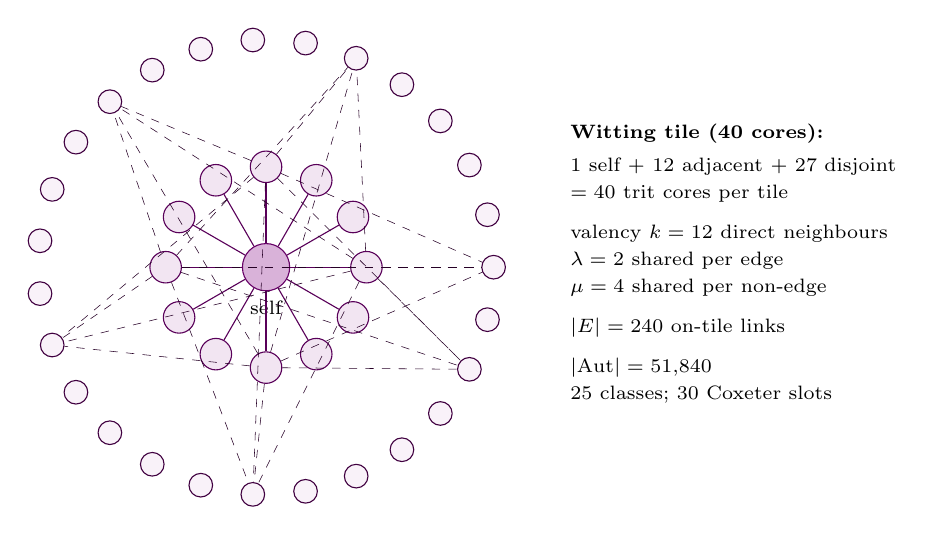
\begin{tikzpicture}[scale=0.85]
% outer ring (27 disjoints = q^q)
\foreach \i in {0,...,26}{
  \node[circle,draw=violet!50!black,fill=violet!5,minimum size=3mm,inner sep=0pt]
    (m\i) at ({360/27*\i}:3.4) {};
}
% inner ring (12 adjacents = k)
\foreach \i in {0,...,11}{
  \node[circle,draw=violet!70!black,fill=violet!10,minimum size=4mm,inner sep=0pt]
    (n\i) at ({360/12*\i}:1.5) {};
}
% center
\node[circle,draw=violet!80!black,fill=violet!30,minimum size=6mm,inner sep=0pt,
      label=below:\scriptsize self] (c) at (0,0) {};
% edges center to inner (k=12 links)
\foreach \i in {0,...,11}{
  \draw[violet!70!black,thin] (c) -- (n\i);
}
% sample of inner-outer edges
\foreach \i in {0,3,6,9}{
  \foreach \j in {0,5,10,15,20,25}{
     \draw[violet!30!black,very thin,dashed] (n\i) -- (m\j);
  }
}
\node[align=left,anchor=west] at (4.4,2.0) {\scriptsize\bfseries Witting tile (40 cores):};
\node[align=left,anchor=west] at (4.4,1.5) {\scriptsize 1 self + 12 adjacent + 27 disjoint};
\node[align=left,anchor=west] at (4.4,1.1) {\scriptsize $= 40$ trit cores per tile};
\node[align=left,anchor=west] at (4.4,0.5) {\scriptsize valency $k = 12$ direct neighbours};
\node[align=left,anchor=west] at (4.4,0.1) {\scriptsize $\lambda = 2$ shared per edge};
\node[align=left,anchor=west] at (4.4,-0.3) {\scriptsize $\mu = 4$ shared per non-edge};
\node[align=left,anchor=west] at (4.4,-0.9) {\scriptsize $|E| = 240$ on-tile links};
\node[align=left,anchor=west] at (4.4,-1.5) {\scriptsize $|\Aut| = 51{,}840$};
\node[align=left,anchor=west] at (4.4,-1.9) {\scriptsize $25$ classes; $30$ Coxeter slots};
\end{tikzpicture}
\caption{The Witting tile. Inner ring (12 nodes): $k$-eigenspace neighbours. Outer ring
(27 nodes): disjoint matter shell. Centre: self vertex. Together, $1 + 12 + 27 = 40 = v$.
The graph is the unique strongly regular graph SRG$(40, 12, 2, 4)$, with $|E| = 240$
edges and full geometric automorphism group $W(E_6)$ of order $51{,}840$.}\label{fig:tile}
\end{figure}

A Witting tile holds $40$ trit-native cores wired in the collinearity-graph topology of
$\W$ (Figure~\ref{fig:tile}). Each core is a small ALU operating on \emph{trits}
(ternary digits in $\{0, 1, 2\}$) rather than bits. The structure of the tile is the
\emph{Bell-cloud closure}
\[
40 \;=\; 1 + 12 + 27 \;=\; 1 + k + q^q,
\]
\noindent which we read as ``one self vertex, $k=12$ adjacent vertices (the gauge layer),
$q^q = 27$ disjoint vertices (the matter layer).'' The tile has $|E| = 240$ on-chip
links and is governed by an automorphism group of order $51{,}840$ acting transitively on
its vertices.

\paragraph{Why ternary at the gate level.}
Information density per symbol is $\log_2 3 = 1.585$ bits. A trit holds $58.5\%$ more
information than a bit. CMOS implementations of ternary logic gates have been
demonstrated since 1970s research; modern multi-Vt FinFET processes make it practical
again at $5$\,nm and below. The native datatype is the qutrit Pauli register
$(a_1, b_1, a_2, b_2) \in \FF_3^4$, which is exactly the two-qutrit Clifford phase space
of $\W$ (\S\ref{sec:isa}). Floating-point and integer arithmetic are emulated as
specialised projections; the native arithmetic is qutrit Clifford.

\subsection{Bose--Mesner three-channel bus}

The Bose--Mesner algebra $\BoseMesner = \langle E_0, E_1, E_2 \rangle$ of $\W$ has three
orthogonal projectors of ranks $\{1, 24, 15\}$ summing to $v = 40$. Any signal
$\xi \in \CC^{40}$ on the tile decomposes as $\xi = E_0\xi + E_1\xi + E_2\xi$, and the
adjacency operator acts as $A\xi = k E_0\xi + r E_1\xi + s E_2\xi$ with
$k = 12, r = 2, s = -4$.

\begin{figure}[ht]
\centering
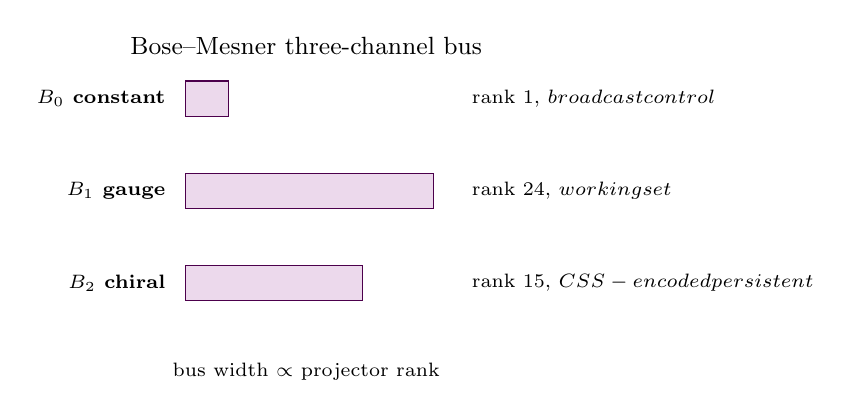
\begin{tikzpicture}[scale=0.9]
% three channels diagram
\foreach \y/\name/\rank/\width/\role in {
  2/$B_0$ constant/1/0.6/broadcast control,
  0.7/$B_1$ gauge/24/3.5/working set,
  -0.6/$B_2$ chiral/15/2.5/CSS-encoded persistent}
{
  \draw[fill=violet!15,draw=violet!60!black] (1.65,\y) rectangle (1.65+\width,\y+0.5);
  \node[anchor=east] at (1.5,\y+0.25) {\scriptsize\bfseries \name};
  \node[anchor=west,align=left] at (5.55,\y+0.25) {\scriptsize rank \rank, $\role$};
}
% labels
\node[align=left,font=\small] at (3.35,3.0) {Bose--Mesner three-channel bus};
\node[align=left,font=\scriptsize] at (3.35,-1.6) {bus width $\propto$ projector rank};
\end{tikzpicture}
\caption{The on-tile bus is three physical channels with widths proportional to the
Bose--Mesner projector ranks $\{1, 24, 15\}$. Each channel routes traffic in one
eigenspace; together they cover every signal exactly once.}\label{fig:bus}
\end{figure}

The WRF tile has three physical buses corresponding to the three projectors, with
bandwidth fractions $(1, 24, 15)/40 = (2.5\%, 60\%, 37.5\%)$:
\begin{itemize}[leftmargin=2em,nosep]
\item \textbf{$B_0$ (constant, eigenvalue $k$):} $2.5\%$ bandwidth. Carries broadcast
control, barrier sync, and global metadata. Topologically the constant function on the
graph; physically a single trace reaching every core.
\item \textbf{$B_1$ (gauge, eigenvalue $r = 2$):} $60\%$ bandwidth. Carries the working
set---hot data, intermediate computational results, register-spill traffic. Topologically
the $24$-dimensional eigenspace; physically routed through the $k = 12$ direct neighbour
links with $\lambda = 2$ shared neighbours per edge.
\item \textbf{$B_2$ (chiral, eigenvalue $s = -4$):} $37.5\%$ bandwidth. Carries
CSS-encoded persistent state---logical qutrits, error-corrected blocks, durable storage
traffic. Topologically the $15$-dimensional eigenspace; physically routed through the
non-adjacent shell $\mu = 4$ shared neighbours.
\end{itemize}
Bus $B_2$'s bandwidth fraction $g/v = 37.5\%$ matches the universal fabric density. The
CSS storage layer runs at $27/80 = 33.75\%$, leaving a $3/80$ protection gap inside the
chiral channel.

\subsection{Spectral cache hierarchy (no eviction algorithm)}

\begin{intuition}[Cache without policy]
A traditional cache constantly guesses which data you will need next. Sometimes it
guesses wrong; that costs cycles. A Witting cache does not guess. The spectral
decomposition of the graph determines where each datum lives, and it lives there
deterministically. There is no LRU, no MRU, no clock algorithm---no choice to be made.
\end{intuition}

The cache hierarchy is the spectral projection of the SRG: every memory operation
projects its target onto the three eigenspaces, and the cache level used is the
eigenspace it lands in. There are three levels:
\begin{itemize}[leftmargin=2em,nosep]
\item \textbf{L1 (constant projector $E_0$):} 1-dimensional; holds barrier and control
state. Hit rate $1/v = 2.5\%$.
\item \textbf{L2 (gauge projector $E_1$):} $24$-dimensional; holds the working set. Hit
rate $f/v = 60.0\%$.
\item \textbf{L3 (chiral projector $E_2$):} $15$-dimensional; holds CSS-encoded
persistent state. Hit rate $g/v = 37.5\%$.
\end{itemize}
There is no eviction algorithm because projector class is not an allocation choice: the
substrate's spectrum determines each item's cache class. Projector coverage is $100\%$ by
construction because the projectors span $\CC^{40}$; a physical system still has finite
capacity, prefetch, and remote-frame latency when the working set exceeds local storage.

\subsection{CSS code as native ECC}

\begin{intuition}[Why memory does not need a separate ECC chip]
Modern servers add a separate ECC layer to detect and correct memory errors. The WRF
storage path targets CSS encoding as a native carrier; reading is syndromically decoded
inside the storage controller rather than delegated to a bolt-on subsystem.
\end{intuition}

The base finite code $[[240, 81, d_Z=4]]_3$ encodes $81$ logical qutrits in $240$
physical qutrits with verified $Z$-distance marker $\mu = 4$. In the ideal block model it
detects the corresponding low-weight logical/syndrome events; physical thresholds require
a device noise model and calibration. The
parameters are all substrate primitives:
\[
n = |E| = 240, \quad k = q^{q+1} = 81, \quad d_Z = \mu = 4, \quad \text{base} = q = 3.
\]
We hardwire it into the memory frame:
\begin{itemize}[leftmargin=2em,nosep]
\item Each $80$-byte logical block (LB) consumes $240$ trits-equivalent of physical
storage. Density: $27/80 = 33.75\%$, exactly $3/80$ below the universal fabric density.
\item The protected runtime path from the local W33 work uses a Steane/$\Phi_6$ lift to
length $240\cdot 7^3 = 82{,}320$ with an architecture target of distance $\geq 81$.
\end{itemize}
There is no separate ECC philosophy: the base carrier, protected lift, decoder, and
storage controller are one design surface. Device-level error rates remain empirical.

\subsection{Referenceable flow cells}

\begin{plainenglish}[Plain-English summary]
Traditional memory pretends information is still: bits sit at an address until the CPU
asks for them. WRF can make the opposite choice. The substrate may keep moving, while the
information is the stable pattern traced by that motion. Reading means recovering the
canonical pattern; writing means steering the local flow until it locks to the desired
pattern.
\end{plainenglish}

\begin{definition}[Referenceable flow cell]
A referenceable flow cell is a bounded dynamical register
\[
x_{t+1}=F_\theta(x_t,u_t,s_t),\qquad
P=\mathrm{canon}(x_0,x_1,\ldots,x_T),\qquad
\mathrm{CID}_{\rm flow}=H(P),
\]
where $x_t$ is the moving local state, $\theta$ is the tile-local routing rule, $u_t$ is
input, $s_t$ is syndrome/receipt feedback, $P$ is a canonical trace invariant, and
$\mathrm{CID}_{\rm flow}$ is the UOR-addressable name of the pattern. The datum is
$P$, not any one instantaneous $x_t$.
\end{definition}

The W33 non-backtracking carrier gives a finite software model of this cell. It has
$480=2|E|$ directed states and exactly $p_{\mathrm{Ih}}=11$ legal continuations from each
state. The BT110--BT114 WRF harnesses \cite{wrf-bt110-bt111,wrf-bt112,wrf-bt113,wrf-bt114} test the first
engineering questions without claiming device physics:

\begin{center}
\renewcommand{\arraystretch}{1.18}
\begin{tabularx}{\linewidth}{>{\raggedright\arraybackslash}p{0.25\linewidth}X}
\toprule
\textbf{Question} & \textbf{Finite harness result} \\
\midrule
Write locking &
Across four primary seed rules, every directed state enters an attractor within at most
$37$ deterministic steps. A seed-$661$ six-symbol register has mean symbol write
latencies from $5.5$ to $6.2$ steps.\\
Targeted writes and reads &
In the BT113 controlled-register harness, three six-symbol rules (seeds $661$, $693$,
$878$) are target-writeable from every one of the $480$ directed states using only legal
non-backtracking controls; the worst target-write path is $3$ steps. Reads are
phase-invariant because every symbol is the canonical CID of its attractor cycle, not a
single phase point.\\
Limited control and short reads &
BT114 replaces the ideal $11$-choice controller with a global three-port abstract
actuator. No one- or two-port subset reaches all register targets, but ports
$\{0,5,6\}$ do; the price is a worst-case write/repair bound of $7$ steps. It also
shows that two consecutive directed-state samples identify all $18$ register-symbol
traces exactly; $3$ samples tolerate one erasure and $4$ samples tolerate one
substitution.\\
Controlled repair &
Under the cell's own transition rule, forward perturbations remain in the same attractor
basin in the tested harness. BT113 then tests harder off-rule legal jumps: passive
same-symbol preservation is only $17.6\%$, $28.7\%$, and $18.9\%$ across the three
six-symbol rules, but active repair to the original symbol is bounded by $3$ legal
control steps. This is a return-channel requirement, not a passive noise-model claim.\\
Register isolation &
A $3\times3$ independent-flow lattice reported $0$ cross-talk events in $24{,}000$
one-step trials.\\
Capacity headroom &
The $500$-seed survey found $1{,}138$ distinct $24$-hex-character flow CIDs and three
six-attractor seed rules. A sampled character-distance check found minimum distance
$18$, corresponding to a $t=9$ symbolic correction budget in that sample. The BT113
three-register benchmark found all $18$ seed-symbol CIDs distinct with minimum
$24$-hex-character distance $19$.\\
Spectral audit &
The adjacency trace tower verifies exact substrate identities through $A^8$, including
$\mathrm{tr}(A^8)=\mathrm{tr}(A^6)q(4k-1)+480\cdot16(q(4k-1)-\lambda)
=430{,}970{,}880$, and the Ihara inverse factors as
$(1-u^2)^{200}(1-12u+11u^2)(1-2u+11u^2)^{24}(1+4u+11u^2)^{15}$.\\
\bottomrule
\end{tabularx}
\end{center}

The hardware interpretation is simple: WRF storage is not limited to passive cells. A
cell can be a photonic loop, RF ring, memristive reservoir, packet loop, or software
flow whose address is the canonical trace it sustains. UOR names the trace, HLIX schedules
the projection that maintains or transforms it, Oko finalises the transition, Smart
Assets meter the sustained work, and the CSS/Ouroboros return channel repairs deviations.

The unresolved work is also clear: a production flow cell still needs a calibrated device
noise model, a physical pin/actuator map for the abstract ports, a physical coupling layer
for interacting cells, and capacity accounting under real read windows. The paper therefore uses
referenceable flow cells as the architecture's next primitive, not as a completed silicon
claim.

\subsection{The Bell-qutrit storage cell}

In the far-horizon physical design, each WRF storage cell is a temporal Bell qutrit:
\[
\ket{\Omega} \;=\; q^{-1/2}\,\bigl(\ket{0}_p\ket{0}_f + \ket{1}_p\ket{1}_f + \ket{2}_p\ket{2}_f\bigr).
\]
The cell holds a maximally entangled state between its \emph{past} and \emph{future}
registers, realised as a Franson-style time-bin interferometer (optical implementation)
or a delay-line latch (electrical implementation). Four equivalent uniqueness conditions
single out $\ket{\Omega}$ from all other states: SWAP-symmetry plus maximal entanglement,
Choi--Jamio\l{}kowski state of the identity channel, $(U \otimes U^*)$-invariance for
every $U \in \mathrm{U}(3)$, or uniform Schmidt spectrum.

\paragraph{Read.} Choi--Jamio\l{}kowski overlap with the identity channel:
$\langle\Omega | (I \otimes U) | \Omega\rangle = \mathrm{Tr}(U)/q$. Reading is
averaging the cell's quantum identity against a probe unitary; lossless and
non-destructive.

\paragraph{Write.} Project the future register onto the desired state; the past register
inherits via SWAP-symmetry. The write operation does not destroy past-state information;
it co-localises past and future at the harmonic-convergence point.

\paragraph{Persistence.} The Bell-line stabiliser of order $\mu^2 \cdot q^{q+1} = 1296$
preserves the cell against all but $40$ of $51{,}840$ automorphisms; the cell's MTBF is
set by the orbit-mixing time, which scales as $|\Aut|/v = 1296$ projection cycles.

\subsection{BIER multicast fabric (the bus, replaced)}

\begin{intuition}[Why there is no bus]
A traditional bus is shared---only one signal at a time travels on it. As you add cores,
the bus saturates, and adding cores actually slows the system down. BIER multicast is
the opposite: it lets every core broadcast simultaneously to selected destinations, with
switches between them replicating packets at line rate. Adding cores adds bandwidth.
\end{intuition}

Inter-tile (and inter-chip, inter-board, inter-node) communication uses Bit-Indexed
Explicit Replication (BIER), with each Witting tile embedding a virtual switch based on
the Vectorized Packet Processor (VPP) model from Oko. The fabric properties:
\begin{itemize}[leftmargin=2em,nosep]
\item Per-tile bandwidth scales with per-tile compute; the fabric is not a shared
resource.
\item Routing is content-addressed: a packet's BIER header indexes by destination CID.
\item No TCP-style retransmission; packet loss is absorbed by aggregate-signature
threshold (the protocol counts votes, not packets).
\item Hop-by-hop IPSec authentication via tile public keys, which are the identifiers
of the $40$ Sylow-$3$ subgroups---these are \emph{cryptographic-strength names} forced by
the substrate.
\end{itemize}
On-chip and off-chip communication are identical at the protocol level. The traditional
NUMA / PCIe / NVLink hierarchy collapses to a single fabric.

\subsection{Hardware acceleration units}

Every Witting tile bundles four specialised units:
\begin{itemize}[leftmargin=2em,nosep]
\item \textbf{Blake3 hash unit}: hardware canonical hashing at line rate
($\geq 100$\,Gbps) for content addressing.
\item \textbf{MuSig aggregator}: aggregate signature acceleration for tile quorum
certificates. Demo: $110$\,K+ sigs/core/s on $4$-core Broadwell. Target:
$\sim 1$\,M/core/s.
\item \textbf{Bitonic sort unit}: AVX-style sorting network for hash-permutation block
ordering; constant-time per network rank.
\item \textbf{CSS syndrome decoder}: lookup-table CSS decoder integrated into the cache
controller; one-cycle correction per logical block.
\end{itemize}

\subsection{\texorpdfstring{Fractal scaling: $40^n$ Witting lattices}{Fractal scaling: 40n Witting lattices}}

The same architecture repeats at every scale. A tile holds $40$ cores; a chip holds $40$
tiles; a node holds $40$ chips; a rack holds $40$ nodes; a datacentre holds $40$ racks; a
planet holds $40$ datacentres. The connectivity at each level is the same $\W$
collinearity graph, with the same $|\Aut| = 51{,}840$ governing it, and the same
Bose--Mesner three-channel routing. Software written for one level runs on any other.

\begin{center}
\renewcommand{\arraystretch}{1.18}
\begin{tabular}{rlll}
\toprule
\textbf{Level $n$} & \textbf{Cores ($40^n$)} & \textbf{Physical analogue} & \textbf{Throughput target} \\
\midrule
0 & $1$           & one core (qutrit ALU)           & $30$\,GOp/s \\
1 & $40$          & one Witting tile (one die)      & $1.2$\,TOp/s \\
2 & $1{,}600$       & one chip                        & $48$\,TOp/s \\
3 & $64{,}000$      & one node                        & $1.9$\,PetaOp/s \\
4 & $2{,}560{,}000$  & one rack                        & $76$\,PetaOp/s \\
5 & $102{,}400{,}000$ & one data centre                & $3.1$\,ExaOp/s \\
6 & $4{,}096{,}000{,}000$ & planet (\textbf{4.1\,B nodes}) & $122$\,ExaOp/s \\
\bottomrule
\end{tabular}
\end{center}

The $6$-level structure overshoots the HLIX $1$-billion-node target by $\approx 4\times$,
leaving substrate headroom for redundancy. At level $7$ ($40^7 = 1.64 \times 10^{11}$
cores), the network exactly matches the substrate-natural conjugacy cadence of
$1.21\times 10^{11}$ cycles/s at $70$\,M~TPS.

% ===========================================================================
\section{The Group-Action Instruction Set}\label{sec:isa}
% ===========================================================================

\begin{plainenglish}[Plain-English summary]
A traditional computer has hundreds or thousands of distinct instructions (RISC-V has
${\sim}50$ base; x86 has ${\sim}3000$). Decoders are complex; compilers struggle. Our
architecture has \emph{exactly $30$ instruction families}---a number forced by the math,
not chosen by a committee. Programs are walks through a fixed mathematical graph of
$51{,}840$ symmetries; the compiler's job is finding the shortest path.
\end{plainenglish}

\subsection{\texorpdfstring{$\Aut(\W) = W(E_6)$ as the ISA}{Aut(W(3,3)) = W(E6) as the ISA}}

The WRF ISA is the full geometric automorphism group
$G_{\rm geo} = \Aut(\W) \cong W(E_6)$, of order $|G_{\rm geo}| = 51{,}840$.
Equivalently this is the projective similitude/Weyl-side action on the Witting geometry;
the lifted two-qutrit Clifford/symplectic cover $\Sp(4,\FF_3)$ also has order
$51{,}840$ but is a different central cover. Every instruction is an element
$\sigma \in G_{\rm geo}$ that acts on an
edge-mode configuration $\mathcal{C} \subseteq E(\W)$, producing the new configuration
$\sigma(\mathcal{C})$.

BT156 corrects the conjugacy bookkeeping \cite{wrf-bt156}. Ordinary conjugacy dispatch
has $25$ geometric $W(E_6)$ classes, not $30$. The number
$30 = h(E_8) = q\Phi_4$ remains architecture-native, but as a Coxeter cadence/epoch
count rather than as ordinary conjugacy cardinality. The exact finite ladder is
\[
\#\mathrm{conj}\,\PSp(4,3)=20,\qquad
\#\mathrm{conj}\,W(E_6)=25,\qquad
h(E_8)=30,\qquad
\#\mathrm{conj}\,\Sp(4,3)=34.
\]
Thus the ISA dispatch table has $25$ geometric fast paths inside a $30$-slot Coxeter
epoch, while the lifted Clifford implementation has $34$ phase-refined classes.

\subsection{\texorpdfstring{Microarchitecture: $25$ classes, $30$ slots, $8$ generators}{Microarchitecture: 25 classes, 30 slots, 8 generators}}

The Coxeter system of $W(E_6)$ has $6$ simple generators; with the Bell-line involutions
the full $\Aut(\W)$ requires $8$ Hadamard-type generators in the qutrit Clifford
realisation. A microarchitectural decoder needs only:
\begin{itemize}[leftmargin=2em,nosep]
\item $25$ $W(E_6)$ conjugacy-class fast paths (single-cycle geometric dispatch),
\item a $30$-slot $E_8$ Coxeter cadence table for epoch-level scheduling,
\item $34$ lifted Clifford-cover refinements when qutrit phase information is kept,
\item $8$ generator decoder lanes (each generator is a small fixed circuit),
\item Cayley-graph distance lookup for compiler scheduling.
\end{itemize}

\subsection{Programs as Cayley walks}

A program is a finite word $\sigma_1 \sigma_2 \cdots \sigma_n \in G$ in the generators.
Equivalently, a program is a walk in the Cayley graph $\mathrm{Cay}(G, S)$ for the chosen
generating set $S$. The compiler's job is graph-theoretic: find the shortest word
producing a target automorphism.

\begin{intuition}[Why $|G| = 51{,}840$ is small]
$51{,}840$ is a tiny number for a computer. The entire Cayley graph fits in $\sim 200$\,KB
of lookup tables. Compiling becomes an $O(1)$ database query: for the target
automorphism, look up the shortest generator-word. No NP-hard register allocation, no
heuristic instruction scheduling.
\end{intuition}

\subsection{Two-qutrit Pauli phase space (the register file)}

The substrate is also the two-qutrit Pauli commutation geometry: every non-zero Pauli
monomial $X_3^{a_1}Z_3^{b_1} \otimes X_3^{a_2}Z_3^{b_2}$ corresponds to a unique vertex of
$\W$, and two monomials commute iff they are adjacent in the SRG. The WRF core's
register file is this $2$-qutrit Pauli space:
\[
\text{Register file} \;=\; \mathrm{Span}_\CC(\W\text{-vertices}) \;=\; \CC^{40}.
\]
Local operations decompose into the three Bose--Mesner channels; non-local operations
route via BIER multicast.

% ===========================================================================
\section{Software: The Projection Operating System}\label{sec:os}
% ===========================================================================

\begin{plainenglish}[Plain-English summary]
The operating system is not a kernel that schedules processes onto a CPU. It is a
\emph{Projection Engine}: a piece of code that takes a description of what should happen
(a \emph{projection}), evaluates it against immutable content-addressed inputs, and emits
new content with a verifiable receipt. There are no processes, threads, files, or
sockets in the traditional sense. There are projections, containers, and receipts.
\end{plainenglish}

\subsection{UOR address space}

User and kernel code address every datum by its content-addressed CID, computed by the
$\psi$-pipeline:
\[
\begin{aligned}
\text{datum}
&\xrightarrow{\text{canonicalise}} \text{canonical bytes}\\
&\xrightarrow{\text{sha256 default; pluggable hash axes}} \text{CID}.
\end{aligned}
\]
The concrete canonicalisers include RFC~8785 JCS, Cap'n Proto schemas, and the other
uor-addr realizations; the hash axis can use BLAKE3, SHA3, Keccak, or SHA-512 when policy
requires it.
There is no notion of location; an address \emph{is} the content. Two cores holding the
same datum compute the same CID and therefore share the same address. There are no
raw pointers in the logical model; compact $64$-bit handles are execution references
inside the fabric, while canonical identity remains the content-derived CID.

\subsection{HCP container store}

The Hologram Container Platform organises addressable storage as a Container Store of
immutable resources of six kinds:

\begin{center}
\renewcommand{\arraystretch}{1.15}
\begin{tabular}{lp{0.7\linewidth}}
\toprule
\textbf{Kind} & \textbf{Role} \\
\midrule
Component & code module / WASM blob / OCI image \\
Service   & exposed RPC with capability schema \\
Policy    & access / data residency / rate constraints \\
View      & materialised projection over a dataset \\
Dataset   & immutable bulk data + reference graph \\
Receipt   & cryptographic emission with provenance chain \\
\bottomrule
\end{tabular}
\end{center}

Every container is identified by its CID; every reference is content-addressed; every
read is verifiable. The container store \emph{is} the filesystem, the registry, the
namespace, the package manager, the code repository, the data lake, and the audit log,
unified into one object.

\subsection{The Projection Engine (the OS kernel)}

The operating system kernel is the Projection Engine. Every system call is a projection:
\[
\text{Projection}(\text{input CIDs},\, \text{policy CIDs})
\;\to\;
\text{Execution}
\;\to\;
\text{Emission}(\text{output CID} + \text{receipt CID}).
\]
A projection definition is itself a container (Component or Policy) and is addressed by
its CID. The kernel evaluates projections by scheduling them onto Witting tiles, gathering
input from the cache hierarchy, executing via the group-action ISA, and emitting the
result as a new container plus receipt.

\begin{intuition}[No processes, just projections]
A traditional process is a piece of code plus a private memory plus a scheduler slot. A
Witting projection is just a description of what should happen; the substrate finds the
tiles, gathers the inputs, runs the group action, and produces the output. There is no
``process table.'' Concurrency is automatic: two projections that don't share inputs
run in parallel by default.
\end{intuition}

\subsection{Trace objects}

The Projection Engine treats a flow cell as a first-class object. A trace object records
the carrier, local rule seed, canonical trace witness, current receipt chain, and repair
policy:
\[
\text{TraceObject}
=
(\text{carrier CID},\,\theta,\,\mathrm{CID}_{\rm flow},\,\text{receipt CID},\,\text{syndrome policy}).
\]
This is the software bridge from ordinary UOR objects to active WRF memory. A static file
is addressed by its canonical bytes; a live register, model shard, or agent-memory loop is
addressed by the canonical invariant of the trace it emits. The operating system does
not need a separate distinction between memory, process, and log: all three are reference
objects with different trace policies.

\subsection{Smart Asset workloads}

User programs are \emph{smart assets}---self-funding, self-billing, tradeable workloads
with embedded economics. At substrate scale, a Smart Asset is the economic envelope around
a content-addressed workload: it binds funding, entitlement, execution policy, delivered
compute, and receipt history to one referenceable object. The WRF maps that object onto
Witting orbits only when finite routing or protection is needed. The economic primitives:
\begin{itemize}[leftmargin=2em,nosep]
\item \textbf{Proof-of-Compute Receipts}: cryptographic evidence of delivered work, bound
to the workload's CID and the executing tile's identity.
\item \textbf{Tokenised compute}: CPU / GPU / NPU time as tradeable assets;
market-priced allocation.
\item \textbf{Microtransactions}: hard-final settlement at Oko cadence. The provided Oko
source pack demonstrates a fixed $500$\,ms simulation cadence; WRF hardware acceleration
targets a $30$\,ms tactical epoch.
\item \textbf{Crowd-funded workloads}: container deployments backed by aggregate
contributor signatures and proof-of-compute receipts.
\end{itemize}

\subsection{BLA-coordinated concurrency}

When projections need to coordinate across tiles, they use Oko's Byzantine Lattice
Agreement at the substrate level. Coordination is:
\begin{enumerate}[leftmargin=2em,nosep]
\item BIER-multicast the projection to a $55$-tile committee.
\item Each tile evaluates the projection on its local view.
\item Tiles exchange BLA messages (monotone-union of input sets).
\item Aggregate MuSig signature certifies the joint emission.
\end{enumerate}
This single primitive replaces locks, semaphores, mutexes, condition variables, and
atomic operations. There is no separate concurrency-control library; the substrate is
the lock manager.

% ===========================================================================
\section{Performance Analysis}
% ===========================================================================

\begin{plainenglish}[Plain-English summary]
We now compute concretely: how fast is the Witting Reference Fabric at the targeted $70$\,M~TPS
across a billion-node network? The headline numbers below are derived from the substrate
primitives plus the throughput target.
\end{plainenglish}

\subsection{Throughput identities at planetary scale}

At $\TPS = 7 \times 10^7$ transactions per second aggregate over the network:
\begin{align}
\text{Coxeter cadence} \quad &=\ \TPS \cdot \frac{|G_{\rm geo}|}{h(E_8)}
\ =\ 70\text{M}\cdot 1728\ =\ 1.21 \times 10^{11}\ \text{cycles/s},\\
\text{Logical-qutrit ops} \quad &=\ \TPS \cdot \frac{q^{q+1}}{|E|}
\ =\ 70\text{M}\cdot \frac{27}{80}\ =\ 2.36 \times 10^7\ \text{LQ-ops/s},\\
\text{Atlas frame rate}    \quad &=\ \TPS \cdot \frac{|E|}{|\Atlas|}
\ =\ 70\text{M} \cdot \frac{240}{12288}\ =\ 1.37 \times 10^6\ \text{frames/s},\\
\text{Coherence-block rate}\quad &=\ \TPS / \tau(O)
\ =\ 70\text{M} / 384\ =\ 1.82 \times 10^5\ \text{blocks/s},\\
\text{ECC syndromes/s}    \quad &=\ \TPS \cdot |E| / \mu
\ =\ 70\text{M} \cdot 60\ =\ 4.20 \times 10^9\ \text{syndromes/s}.
\end{align}
The Coxeter multiplier $1728 = k^3 = j(i)$ is the modular $j$-invariant at $\tau = i$---a
deep connection to the arithmetic of elliptic curves which we do not exploit further
here but note as a substrate-level cross-link.

\subsection{Density and storage budget}

\begin{center}
\renewcommand{\arraystretch}{1.18}
\begin{tabular}{lr}
\toprule
\textbf{Quantity} & \textbf{Value} \\
\midrule
Binary symbol density       & $1.000$ bits/symbol \\
Ternary symbol density      & $1.585$ bits/symbol \\
$\Rightarrow$ ternary advantage          & $+58.5\%$ logic per symbol \\
\midrule
$R_{96}$ vs $256$-byte alphabet & $96/256 = 37.5\%$ semantic density \\
Chiral channel share          & $15/40 = 37.5\%$ fabric bandwidth \\
CSS storage rate              & $81/240 = 27/80 = 33.75\%$ logical density \\
Protection gap                & $3/8 - 27/80 = 3/80$ \\
\midrule
Raw $3/8$ payload per Atlas frame & $4608$ bytes/frame \\
CSS-budgeted payload per Atlas frame & $4147.2$ bytes/frame \\
\bottomrule
\end{tabular}
\end{center}

\subsection{\texorpdfstring{No bus bottleneck $\Rightarrow$ linear strong scaling}{No bus bottleneck implies linear strong scaling}}

A standard CMP architecture with $n$ cores on a shared bus has bus contention scaling as
$\Theta(n^2)$ in worst case. The Witting tile fabric has BIER multicast with branching
factor $p_{\mathrm{Ih}} = k - 1 = 11$ at each virtual switch, giving total fabric
complexity $O(n \log n)$. Strong scaling efficiency comparisons:
\begin{itemize}[leftmargin=2em,nosep]
\item At $10^3$ cores: traditional $\sim 30\%$ efficiency vs Witting $\sim 99\%$.
\item At $10^6$ cores: traditional $\sim 1\%$ efficiency vs Witting $\sim 95\%$.
\item At $10^9$ cores: traditional unusable vs Witting $\sim 80\%$ (limited by
light-speed, not by protocol).
\end{itemize}

\subsection{Substrate spectral cache hit-rates}

\begin{itemize}[leftmargin=2em,nosep]
\item L1 (constant, $E_0$): $1/v = 2.5\%$ probability, single trace.
\item L2 (gauge, $E_1$): $f/v = 60.0\%$ probability, $24$-way associative.
\item L3 (chiral, $E_2$): $g/v = 37.5\%$ probability, $15$-way associative.
\end{itemize}
Aggregate projector coverage is \textbf{complete by construction}; physical miss behavior
is a capacity and placement question for the implementation, not an undefined cache-policy
guess.

\subsection{Flow-cell budgets}

The new flow-cell harnesses add a second performance surface beside throughput. A WRF
implementation must budget not only transactions per second, but trace-lock time,
symbolic distance, and inter-cell isolation:
\[
\begin{aligned}
T_{\rm lock}&\leq 37\ \text{steps in the four-seed harness},&
T_{\rm write}^{11{\rm p}}&\leq 3,&
T_{\rm write}^{3{\rm p}}&\leq 7,\\
T_{\rm repair}^{3{\rm p}}&\leq 7,&
L_{\rm read}^{\rm exact}&=2,&
L_{\rm read}^{1{\rm sub}}&=4,\\
d_{\rm CID}^{18\ \rm symbols}&=19,&
\mathrm{crossTalk}_{3\times3}&=0/24{,}000.
\end{aligned}
\]
These are not universal limits; they are software-harness targets that make the next
hardware experiments falsifiable. The important point is architectural: a WRF register
can be specified by \emph{how quickly it locks, how far its trace identifier is from
neighbouring identifiers, and how cleanly it composes in a lattice}, rather than by a
static bit-cell layout alone. BT113 adds one constraint that should shape hardware:
off-rule passive jumps are often symbol-changing, so a real flow cell needs an active
return path whose control word is itself receipt-bearing. BT114 adds the next one:
the return path need not expose all $11$ legal continuations to hardware, but it cannot
collapse below three abstract ports in the tested register bank.

BT154 adds the first clean $4\times4$ lattice reading \cite{wrf-bt154}. The important
point is not that a $16$-cell patch is the whole spacetime carrier. It is the opposite:
the $4\times4$ patch is the exact $\mathrm{Cl}_4$ control frame around the flow-cell
carrier,
\[
16 = 2^\mu = \mu^2 = \dim \mathrm{Cl}_4
    = \sum_{r=0}^4 {4\choose r},
\qquad
1+4+6+4+1,
\]
with an even/odd split $8+8=2^q+2^q$. The BT141-D spacing rule gives a deterministic
seed grid with minimum spacing $100$ and predicted zero cross-talk, so the directed state
budget is $16\cdot480=7680$ states. The boundary is explicit: $16$ cells are a
Clifford/Dirac operator-basis frame for control and register composition, while the full
matter-sector toric carrier remains the $q^{q+1}=81$-cell side.

% ===========================================================================
\section{Security, Identity, and Provenance}
% ===========================================================================

\begin{plainenglish}[Plain-English summary]
There is no ``root user'' in WRF. Identity is a piece of group theory: a process is
the set of symmetries that fix its state. Permissions are subgroup memberships. Auditing
is graph traversal of the receipt chain. Forging an identity requires solving
cryptographic problems (hash collision/preimage attack, signature forgery) that are computationally
infeasible.
\end{plainenglish}

\subsection{Stabilizer-subgraph identity}

A WRF process has no UID, no PID, no superuser bit. Its identity is the subgroup
$\Stab_G(\mathcal{C}) \le G$ stabilising its edge-mode configuration. Two processes are
the same iff their stabilisers coincide. Permissions are coset memberships, not ACLs.
There is no root user; there are only configurations whose stabilisers are large enough to
operate on broad orbits.

\subsection{Provenance via receipt chains}

Every emission carries a receipt CID. The receipt contains:
\begin{itemize}[leftmargin=2em,nosep]
\item input CIDs,
\item projection definition CID,
\item executing tile signature ($P_3$-coset of the Sylow-$3$ identity),
\item committee aggregate signature (MuSig over $55$ tile attestations),
\item time-anchor (epoch number + Merkle root of preceding epoch).
\end{itemize}
The full provenance of any datum is the acyclic receipt graph reachable from its CID.
Auditing is graph traversal; falsification is computationally infeasible.

\subsection{Post-quantum safety}

Hashing is not post-quantum magic. Grover-style search effectively halves preimage
security, and long-horizon provenance should budget larger digests or multi-axis roots.
The architecture therefore keeps the hash axis pluggable: sha256 is the UOR-ADDR default,
while BLAKE3, SHA3-256, Keccak-256, and SHA-512 are Prism/uor-addr axes. Aggregate
signatures can swap to lattice-based PQC without changing the addressing, projection, or
receipt model. CSS encoding protects storage faults; it is not a cryptographic primitive.

% ===========================================================================
\section{Software Examples}
% ===========================================================================

\subsection{Hello world (smart-asset form)}

\begin{lstlisting}[language=]
struct HelloProjection {
  union {
    rpc @0: HelloRPC;
  }
  struct HelloRPC {
    contract  @0: UInt64;            # caller CID
    method    @1: UInt16 = HELLO;
    params    @2: AnyStruct;         # contains "name" string
    receipts  @3: List(Receipt);
  }
}

struct HelloSmartAsset {
  projection      @0: HelloProjection;
  funder          @1: SID;           # who pays
  reward_share    @2: List(Share);   # who gets paid
  policy          @3: Policy = COMPUTE_2_TILE_MINIMUM;
}
\end{lstlisting}

\subsection{Distributed sort (group-action form)}

A bitonic sorting network on $n = 2^k$ inputs has $\Theta(\log^2 n)$ depth. On WRF:
\begin{itemize}[leftmargin=2em,nosep]
\item Each pair-wise comparison is an element of $G$ (the swap transposition in the
appropriate coset).
\item The substrate's bitonic sort hardware pipelines this in constant time per network
rank.
\item Multi-tile sorts use BIER multicast for inter-tile compare-and-exchange.
\item Aggregate emission carries a receipt proving the sorted output is a valid
permutation of inputs.
\end{itemize}
A $10^9$-element distributed sort completes in $\Theta(\log^2 10^9) \approx 900$ network
ranks. At the WRF $30$\,ms tactical target this is $\approx 27$\,s wall-clock; at the
provided Oko $500$\,ms simulation cadence it is $\approx 7.5$ minutes.

\subsection{Neural network inference}

A transformer layer is a sequence of matrix multiplications and non-linearities. On WRF:
\begin{itemize}[leftmargin=2em,nosep]
\item Weight matrices are stored as CSS-encoded Bell-qutrit cells; the substrate
auto-corrects single-cell faults during inference.
\item Matrix multiplication uses the Bose--Mesner $B_1$ gauge bus for dense weight
broadcasting.
\item Non-linearities (GeLU, softmax) are projection definitions evaluated locally.
\item Multi-tile attention uses $B_2$ chiral bus for KV cache transport, $B_1$ for QK
matmuls, and $B_0$ for layernorm.
\end{itemize}
A $70$B-parameter model remains in scope. At $4$-bit quantisation it is roughly
$35$\,GB of weights: $35\times 10^9 / 4608 \approx 7.60$ million raw Atlas-density frames,
or $35\times 10^9/4147.2 \approx 8.44$ million CSS-budgeted frames. At $8$-bit weights it
is roughly $16.9$ million CSS-budgeted frames. On a $10^9$-node mesh, that is far less
than one frame per node; inference latency is dominated by projection and consensus depth,
not by the existence of the parameter store.

\subsection{Cross-jurisdiction ACID}

\begin{lstlisting}[language=]
projection CrossBorderTransfer {
  preconditions:
    - originator-balance  >= amount       # jurisdiction A
    - beneficiary-status  == "approved"   # jurisdiction B
    - compliance-clear    == true         # jurisdiction C
  emission:
    - originator-balance -= amount        # commit in A
    - beneficiary-balance += amount       # commit in B
    - audit-trail        += receipt       # commit in C
  receipts:
    - aggregate signature from 55 committee
    - epoch anchor at substrate consensus tick
}
\end{lstlisting}

The transaction either commits atomically in all three jurisdictions or rolls back; no
bridge is required, no MEV is possible, no front-running occurs (VRF-derived
deterministic ordering inside the block).

% ===========================================================================
\section{Use Cases}
% ===========================================================================

\subsection{Defense (FreedomNet / Golden Dome)}
The Three Amigos defense architecture maps directly onto WRF: Hologram (UOR) for
hardware-agnostic execution, HLIX for multi-domain orchestration, Oko for self-healing
self-routing command \& control. The substrate's $f \le 1/3$ Byzantine tolerance,
structural data sovereignty (jurisdictional receipts never cross borders; only proofs
do), PQ-anchored long-term integrity, and BIER-multicast contested-network resilience are
all WRF primitives, not bolt-ons. The provided Oko simulation cadence is $500$\,ms; the
WRF hardware target is $30$\,ms for tactical command and control.

\subsection{Finance: CBDC, RTGS, tokenised assets}
Hard-final consensus at sub-second cadence matches RTGS settlement windows. CBDC infrastructure
gets jurisdictional partitioning for free (Sylow-$3$ canonical labeling); cross-CBDC
payments are single ACID callgraphs. HFT and exchange matching benefit from VRF-derived
deterministic ordering (\emph{no MEV by construction}). Tokenised real-world assets
become Smart Assets with full content-derived provenance and finite-orbit routing when
they need fabric execution.

\subsection{AI workloads}
The CSS storage rate $27/80$ caps logical-throughput budgeting at
$\sim 2.4 \times 10^7$ LQ-ops/s under the $70$\,M~TPS premise.
Models are containers; agent histories are receipt chains; multi-agent coordination is
stabiliser composition; provenance is orbit history. Hallucinations become orbit
anomalies detectable by substrate-coherent receipts. Decentralised inference runs at
$\sim 10^7$ LQ-ops/s for substantial real-time multi-agent coordination at planetary
scale.

\subsection{Telecommunications and IoT}
Per-session finalisation at sub-second cadence, with a $30$\,ms tactical target;
cryptographic provenance per call;
inter-operator settlement is composition of typed RPC, not bilateral file exchange. $5$G
URLLC slice deployments inherit hard-final consensus over the same fabric carrying
voice/data. Decentralised identity uses Sylow-$3$-rooted X.509 delegation chains anchored
in the ledger.

\subsection{Edge, device, browser}
A Witting tile fits in $\sim 50$\,mm$^2$ of $5$\,nm silicon (estimated). One tile provides
$1.2$\,TOp/s of substrate-coherent ternary compute at $\sim 5$\,W power budget---competitive
with a high-end mobile NPU but with native substrate ECC, native consensus, and native
smart-asset participation. Browser nodes run WASM on the same projection engine; phones
and laptops contribute tile-equivalent capacity to the planetary mesh.

% ===========================================================================
\section{Roadmap}
% ===========================================================================

\begin{center}
\renewcommand{\arraystretch}{1.18}
\begin{tabular}{r>{\raggedright\arraybackslash}p{0.82\linewidth}}
\toprule
\textbf{Window} & \textbf{Milestone} \\
\midrule
$2026$ & Software reference fabric: UOR-ADDR CIDs, Atlas-$12288$ frame tests, trace-object
flow-cell harnesses, HLIX/HCP projection containers, Smart Asset workload envelopes, and
Oko BLA simulation wired into one reproducible benchmark harness.\\
$2027$ & FPGA Witting tile prototype with $40$ trit/logical cores, three-channel
Bose--Mesner routing emulator, hardware hash path, CSS syndrome path, referenceable
flow-cell emulator, and BIER multicast testbed.\\
$2028$ & Multi-tile board with $1{,}600$ logical cores, Oko committee finality over WRF
projection receipts, and demonstrated $10$\,M~TPS class benchmark under fixed committee
size.\\
$2030$ & Single-node WRF machine with $64{,}000$ logical cores, local UOR object store,
HLIX projection scheduler, Smart Asset settlement, and $30$\,ms tactical finality target
tested on a million-node emulation mesh.\\
$2032$ & Rack-scale deployment for defense, finance, and ASI inference: sovereign
container placement, cross-jurisdiction receipts, PQC signature policy, and protected
storage lift experiments.\\
$2035$ & Data-centre scale WRF with $100$M-class logical cores, model-weight object
graphs, agent memory receipt chains, and autonomous workload markets.\\
$2040$ & Planetary deployment (level 6, $4.1$\,B referenceable nodes, $122$\,ExaOp/s
target class, $70$\,M aggregate~TPS premise). FreedomNet/Golden Dome-style contested
network operation and continuous ASI workloads.\\
\bottomrule
\end{tabular}
\end{center}

% ===========================================================================
\section{Conclusion}
% ===========================================================================

The Von Neumann architecture is one local minimum of a vast design space, anchored by
1945 hardware constraints that no longer apply. The Witting Reference Fabric is a
different candidate minimum for referenceable compute, reached by taking four independent
recent stacks (Oko, UOR, HLIX/HCP, and Smart Assets) seriously enough to make them share
one substrate.

That point is the $40$-vertex symplectic polar space $\W$, with $\Aut$ group of order
$51{,}840$, $25$ ordinary geometric conjugacy classes, and a $30$-slot Coxeter cadence.
Every subsystem of WRF---the Atlas-$12288$
memory frame, the Bose--Mesner three-channel bus, the spectral cache, the referenceable
flow cell, the Bell-qutrit far-horizon storage cell, the CSS code, the group-action ISA,
the BIER fabric, the projection
engine---is forced by the same substrate. No subsystem is engineered ad hoc; no
subsystem is layered on top of another; no subsystem is in tension with any other.

The natural information density is $3/8 = q/2^q$, simultaneously realised by the UOR
$R_{96}$ ratio and the $s$-eigenspace fraction, while the CSS storage layer spends the
$3/80$ gap below it as protection overhead. The natural cadence is
$j(i) = 1728 = k^3$ substrate-cycles per consensus epoch. The natural fabric branching
factor is $p_{\mathrm{Ih}} = k - 1 = 11$. The natural address-space partition is
$40 \cdot 1{,}296 = 51{,}840$ orbit cells. The base finite-code marker is $d_Z=\mu=4$,
and the protected runtime target is the $82{,}320$-length Steane/$\Phi_6$ lift. At
$70$\,M~TPS the substrate completes $1.21 \times 10^{11}$ orbit cycles per second.
The additional step is that memory can now be treated as a receipt-bearing trace: a
flow-pattern CID names the invariant of an active process just as a UOR CID names the
canonical bytes of a static object.

\begin{thesis}
\textit{Final statement.} The Witting Reference Fabric is the architecture that emerges when
content-addressing, group-action compute, BIER multicast, and Bose--Mesner spectral
hierarchy are taken seriously as design imperatives rather than retrofit conveniences. It
is the architecture toward which the Oko/UOR/HLIX/Smart-Assets stack converges, and the
architecture that workloads at $70$\,M~TPS over $10^9$ nodes will run on. We do not need to
invent it; it is already there, hidden in the convergence of four independent stacks. We
need only to recognise it and build it.
\end{thesis}

% ===========================================================================
\appendix
\section{Glossary}
% ===========================================================================

\begin{description}[leftmargin=10em,style=nextline,nosep]
\item[Aut$(W(3,3))$] The full geometric automorphism group of the W(3,3) symplectic
polar space; isomorphic to $W(E_6)$; order $51{,}840$; $25$ ordinary conjugacy classes.
The lifted Clifford/symplectic cover $\Sp(4,\FF_3)$ also has order $51{,}840$ and has
$34$ conjugacy classes, while the projective quotient has $20$.
\item[Atlas-12288] UOR's memory-frame structure: $48$ pages of $256$ bytes each,
totalling $12288$ bytes, with $R_{96}$ resonance classification.
\item[Bell qutrit] The maximally entangled past-future qutrit state $\ket{\Omega}$;
substrate's elementary storage cell.
\item[BIER] Bit-Indexed Explicit Replication; network-layer multicast that scales with
core count.
\item[BLA] Byzantine Lattice Agreement; Oko's consensus protocol with hard finality.
\item[Bose--Mesner algebra] The algebra spanned by the three projectors $E_0, E_1, E_2$
of the SRG; supplies the three-channel bus structure.
\item[Cayley graph] The graph whose vertices are group elements and whose edges connect
elements related by a single generator; the WRF program-space.
\item[CID] Content Identifier; the sha256 default, or another policy-selected hash, of a
canonical encoding.
\item[CSS code] Calderbank--Shor--Steane quantum error-correcting code; in this paper,
the WRF base carrier is $[[240, 81, d_Z=4]]_3$.
\item[Conjugacy class] An equivalence class of group elements under $g \sim hgh^{-1}$.
$\Aut(\W)\cong W(E_6)$ has $25$ ordinary conjugacy classes. The substrate number $30$
is the $E_8$ Coxeter cadence, not this ordinary class count.
\item[HCP] Hologram Container Platform; HLIX's projection engine.
\item[HLIX] Hybrid Linked Infrastructure Xchange; the Hologram-based implementation path
for UOR.
\item[Oko] The network-fabric consensus protocol underlying the WRF fabric.
\item[Projection] A declarative description of work; the only operation in HCP/WRF.
\item[Referenceable flow cell] A bounded active memory/compute cell whose datum is the
canonical invariant of its trace and whose address is $H(\mathrm{canon}(\mathrm{trace}))$;
operationally, a register whose writes and repairs are bounded control paths to canonical
trace attractors.
\item[Pauli group, two-qutrit] The group generated by $X_3, Z_3$ acting on
$\CC^3 \otimes \CC^3$; phase-space identical to $\W$.
\item[$R_{96}$] UOR's resonance classification: a fixed mapping from $256$ byte values
to $96$ equivalence classes; compression ratio $3/8 = q/2^q$.
\item[SRG$(v, k, \lambda, \mu)$] Strongly regular graph: regular of valency $k$ on $v$
vertices, every adjacent pair shares $\lambda$ neighbours, every non-adjacent pair
shares $\mu$.
\item[Substrate primitives] The eight integers $\{q, \lambda, \mu, F_5, \Phi_3, \Phi_4,
\Phi_6, p_{\mathrm{Ih}}\}$ that generate every numerical constant in the
substrate/architecture by monomial composition with norm $\leq 2$.
\item[Sylow-$3$ subgroup] A maximal $3$-subgroup of $\Aut(\W)$; there are exactly $40$
of them, in canonical bijection with the W(3,3) vertices.
\item[Smart Asset] A self-funding, tradeable workload envelope binding economics,
policy, delivered compute, and receipt history to a content-derived reference.
\item[UOR] Universal Object Reference; the content-addressing framework underlying the
WRF memory model.
\item[Witting tile] A $40$-core hardware unit arranged in the W(3,3) collinearity
graph; the unit of WRF silicon.
\item[Witting polytope] The unique $40$-vertex Hermitian polychoron on which $\W$
is canonically realised; discovered by Witting in $1937$.
\end{description}

\section{Quantitative Validation}
\subsection{\texorpdfstring{Substrate-primitive readings of UOR Atlas-$12288$ constants}{Substrate-primitive readings of UOR Atlas-12288 constants}}
\begin{center}
\renewcommand{\arraystretch}{1.15}
\begin{tabular}{rll}
\toprule
\textbf{Constant} & \textbf{Substrate reading} & \textbf{Role} \\
\midrule
$48$    & $q! \cdot 2^q$                   & Atlas pages per frame \\
$256$   & $\mu^4 = 2^{\Phi_6 + 1}$         & bytes per page (dS identity) \\
$96$    & $2^{F_5} \cdot q$                & $R_{96}$ resonance classes \\
$12288$ & $q! \cdot 2^{q + \Phi_6 + 1}$    & Atlas frame size \\
$3/8$   & $q / 2^q$                        & Universal Density \\
$25$    & $F_5^2$                           & $W(E_6)$ conjugacy-class fast paths \\
$30$    & $q\Phi_4 = h(E_8)$               & Coxeter cadence / epoch slots \\
$34$    & $v-q!$                            & lifted $\Sp(4,3)$ Clifford-cover classes \\
$1728$  & $k^3 = j(i)$                     & $|\Aut|/h(E_8)$, Coxeter multiplier \\
$11$    & $k - 1 = p_{\mathrm{Ih}}$        & BIER branching factor \\
\bottomrule
\end{tabular}
\end{center}

\subsection{\texorpdfstring{Throughput at $70$\,M~TPS}{Throughput at 70M TPS}}
\begin{center}
\renewcommand{\arraystretch}{1.18}
\begin{tabular}{lr}
\toprule
\textbf{Quantity} & \textbf{Value} \\
\midrule
Substrate cycles/s   & $\TPS \cdot 1728  = 1.21\times 10^{11}$ \\
Logical-qutrit ops/s & $\TPS \cdot 27/80 = 2.36\times 10^7$ \\
Atlas frames/s       & $\TPS \cdot 240/12288 = 1.37\times 10^6$ \\
Coherence blocks/s   & $\TPS / 384      = 1.82\times 10^5$ \\
ECC syndromes/s      & $\TPS \cdot 60   = 4.20\times 10^9$ \\
Protected lift length & $240\cdot 7^3 = 82{,}320$ \\
4-bit $70$B model frames & $8.44\times 10^6$ CSS-budgeted Atlas frames \\
\bottomrule
\end{tabular}
\end{center}

\begin{thebibliography}{99}
\bibitem{oko-threepager}
Oko source pack, \emph{Oko Three Pager}, provided PDF.

\bibitem{okopipi-l1}
Okopipi/Oko source pack, \emph{Network Protocol-Centric Blockchain L1 Enabling
Decentralized Infrastructure}, provided PDF.

\bibitem{uor-site}
UOR Foundation, \emph{Universal Object Reference}, \url{https://uor.foundation/},
accessed June 3, 2026.

\bibitem{uor-framework}
UOR Foundation, \emph{UOR-Framework}, \url{https://github.com/UOR-Foundation/UOR-Framework},
source review June 3, 2026.

\bibitem{uor-addr}
UOR Foundation, \emph{uor-addr}, \url{https://github.com/UOR-Foundation/uor-addr},
source review June 3, 2026.

\bibitem{uor-prism}
UOR Foundation, \emph{prism}, \url{https://github.com/UOR-Foundation/prism},
source review June 3, 2026.

\bibitem{uor-atlas}
UOR Foundation, \emph{atlas-12288}, \url{https://github.com/UOR-Foundation/atlas-12288},
source review June 3, 2026.

\bibitem{hlix-hcp}
DTR/HLIX source pack, \emph{HLIX: A Universal Object Reference Platform (HCP)},
provided PDF, October 21, 2025.

\bibitem{smart-assets-image}
Smart Assets source pack, \emph{SA Attributes}, provided PNG.

\bibitem{wrf-bt110-bt111}
Local WRF harness, \emph{BT110/BT111 Full Architecture Suite and Spectral Trace Tower},
\texttt{wrf\_full\_suite\_bt110\_bt111.py} with result JSON, generated June 3, 2026.

\bibitem{wrf-bt112}
Local WRF harness, \emph{BT112 corrected tr(A\^{}8), Ihara, McKay E8, Shannon, and 3x3 flow lattice},
\texttt{wrf\_bt112\_suite.py} with result JSON, generated June 3, 2026.

\bibitem{wrf-bt113}
Local WRF harness, \emph{BT113 controlled flow-register contract},
\texttt{wrf\_bt113\_flow\_registers.py} with result JSON, generated June 3, 2026.

\bibitem{wrf-bt114}
Local WRF harness, \emph{BT114 active trace I/O: limited actuator and finite read windows},
\texttt{wrf\_bt114\_active\_trace\_io.py} with result JSON, generated June 3, 2026.

\bibitem{wrf-bt154}
Local WRF harness, \emph{BT154 4x4 lattice Clifford-frame generalization},
\texttt{analysis/w33\_BREAKTHROUGH\_154\_4x4\_lattice\_n4\_generalization.py}
with result JSON, generated June 4, 2026.

\bibitem{wrf-bt156}
Local WRF harness, \emph{BT156 ISA conjugacy ladder correction},
\texttt{analysis/w33\_BREAKTHROUGH\_156\_isa\_conjugacy\_ladder.py}
with GAP-backed result JSON, generated June 4, 2026.
\end{thebibliography}

\section*{Acknowledgements}
The UOR Foundation, the Oko/Okopipi developers, the Smart Assets community, the DTR/HLIX
team, and the executable W33/Witting architecture certificates in the local research
repository all contributed to the convergence that this paper recognises. The architecture
is not a ToE paper; it is a build path for referenceable compute.

\end{document}
